\documentclass{beamer}
\hypersetup{unicode}
\usepackage[utf8]{inputenc}
%\usepackage[T1]{fontenc}
\usepackage[croatian]{babel}
\usepackage{csquotes}
\MakeOuterQuote{"}
\usepackage{thmtools}

\declaretheorem{teorem}
% \numberwithin{teorem}{section}
% \numberwithin{equation}{section}
% \numberwithin{figure}{section}
% \numberwithin{table}{section}
\declaretheorem[sibling=teorem, style=plain]{lema}
\declaretheorem[style=remark, sibling=teorem]{napomena}
\declaretheorem[style=remark, sibling=teorem]{komentar}
\declaretheorem[style=definition, sibling=teorem]{definicija}
\declaretheorem[sibling=teorem]{korolar}
\declaretheorem[style=remark, sibling=teorem]{zadatak}
\declaretheorem[sibling=teorem]{propozicija}
\declaretheorem[style = example]{primjer}

\usepackage[
%	style=alphabetic,
%	style=numeric,
style=authoryear,
	giveninits
	% firstinits=true,
	% terseinits=true,
	% giveninits=true
]{biblatex}
\addbibresource{literatura-prez.bib}
\usepackage{tikz}

\usepackage{listings}
\usepackage{booktabs}


% manage colors: https://www.r-bloggers.com/2011/11/create-your-own-beamer-template/
% and https://ramblingacademic.com/2015/12/08/how-to-quickly-overhaul-beamer-colors/

\usetikzlibrary{arrows}
\newcommand{\midarrow}{\tikz \draw[-triangle 90] (0,0) -- +(.1,0);}

% 225fb9, 238947?
% orig 21b2aa b2217f
% dobar zeleno-ljubicasti par 309030-903090
\definecolor{seagreen}{HTML}{309030}
\definecolor{magenta}{HTML}{903090}
\definecolor{gold}{HTML}{ca9520}
\definecolor{red}{HTML}{da272f}
\definecolor{blue}{HTML}{4682b4}
\definecolor{purple}{HTML}{a65cef}

\definecolor{white}{HTML}{ffffff}
\definecolor{dwhite}{HTML}{eeeeee}
\definecolor{black}{HTML}{000000}
\definecolor{lblack}{HTML}{222222}

\colorlet{bgmain}{seagreen}
\colorlet{bgsec}{magenta}
\colorlet{bgter}{gold}
\colorlet{fgmain}{black}
\colorlet{fgsec}{lblack}

\usetheme{Madrid}
\usecolortheme{spruce}
% \useinnertheme{rounded}

% \setbeamercolor{titlelike}{parent=structure, bg=seagreen, fg=white}
% \setbeamercolor{palette primary}{bg=magenta, fg=white}
% \setbeamercolor{palette secondary}{bg=magenta, fg=white}
% \setbeamercolor{palette tertiary}{bg=magenta, fg=white}
% \setbeamercolor{palette quaternary}{bg=magenta, fg=white}
% \setbeamercolor{structure}{bg=white, fg=magenta} % itemize, enumerate, etc
% \setbeamercolor{section in toc}{fg=black, bg=lblack} % TOC sections
% \setbeamercolor{frametitle}{fg=white, bg=seagreen}

% \setbeamercolor{block title}{fg=white, bg=seagreen}
% % \setbeamercolor{block body}{bg=white, fg=white}

% % \usepackage{hyperref}
% % \hypersetup{
% %     colorlinks=true,
% %     urlcolor=magenta
% % }

% % Override palette coloring with secondary
% \setbeamercolor{subsection in head/foot}{bg=seagreen,fg=white}

\lstdefinestyle{mystyle}{
	backgroundcolor=\color{white},
	commentstyle=\color{magenta},
	keywordstyle=\color{seagreen},
	stringstyle=\color{magenta},
	basicstyle=\ttfamily\footnotesize,
	breakatwhitespace=false,
	breaklines=true,
	captionpos=b,
	keepspaces=true,
	numbers=none,
	showspaces=false,
	showstringspaces=false,
	showtabs=false,
	tabsize=2
}
\lstset{style=mystyle}

\renewcommand{\mathrm}[1]{\mathsf{#1}}
\newcommand{\ub}{\rightarrow \infty}
\newcommand{\un}{\rightarrow 0}
\newcommand{\norm}[1]{\left\lVert#1\right\rVert} 
\newcommand{\dotnorm}{\left\lVert \, \cdot \, \right\rVert}
% \newcommand{\given}{\, \middle\vert \,}
\newcommand{\given}{\, \vert \,}
\newcommand{\st}{\, \colon \,}
\newcommand{\D}{\,\mathrm d}
\newcommand{\ani}{{^\perp}}
\newcommand{\ran}{\mathrm{ran}\,}
\newcommand{\bop}{\mathrm{B}}
\newcommand{\skp}[2]{\left\langle {#1}, {#2}  \right\rangle}
\newcommand{\jpod}{\stackrel{\mathrm d}{=}}
\newcommand{\jgs}{\stackrel{\mathrm{g.s.}}{=\joinrel=}}
%\newcommand{\jzbog}[1]{\stackrel{\eqref{#1}}{=}}
\newcommand{\stackrell}[2]{\stackrel{\scriptstyle {#1}}{#2}}
\newcommand{\konvp}{\stackrel{\mathbb P}{\longrightarrow}}
\newcommand{\konvw}{\stackrel{\mathrm w}{\longrightarrow}}
\newcommand{\konvd}{\stackrel{\mathrm d}{\longrightarrow}}
\newcommand{\konvgs}{\stackrel{\mathrm{g.s.}}{\longrightarrow}}
\DeclareMathOperator{\card}{card}
\DeclareMathOperator{\var}{Var}
\DeclareMathOperator{\supp}{supp}
\DeclareMathOperator{\im}{im}
\DeclareMathOperator{\olspan}{\overline{span}}
\DeclareMathOperator{\re}{Re}
\DeclareMathOperator{\sgn}{sgn}

\newcommand{\ol}[1]{\overline{#1}}
\newcommand{\wh}[1]{\widehat{#1}}
\newcommand{\wt}[1]{\widetilde{#1}}
\renewcommand{\th}[1]{\hat{#1}} % drukciji hat za tekst?
% \newcommand{\eqdef}{\ {=\colon} \ } 
% \newcommand{\defeq}{\ {\colon\!=} \ }

\newcommand{\R}{\mathbb{R}}
\newcommand{\N}{\mathbb{N}}
\newcommand{\Z}{\mathbb{Z}}
\newcommand{\Q}{\mathbb{Q}}
\newcommand{\C}{\mathbb{C}}
\renewcommand{\P}{\mathbb{P}}
\newcommand{\Ptrans}{\P}  % trazicijska funkcija Markovljevog procesa
\newcommand{\E}{\mathbb{E}}
\def\B{\mathrm{B}}
\def\K{\mathrm{K}}
\def\M{\mathrm{M}}
\def\CC{\mathrm{C}}
\def\RR{\mathrm{R}}
\def\H{\mathcal{H}}
\def\K{\mathcal{K}}
% \def\Z{\mathcal{Z}}
\def\S{\mathcal{S}}
\def\T{\mathcal{T}}
\def\U{\mathcal{U}}

\newcommand{\cz}{Calder\' on--Zygmund}
\newcommand{\holder}{H\" older}
\newcommand{\cadlag}{c\` adl\` ag}
\newcommand{\levy}{L\' evy}
\newcommand{\ito}{It\= o}
\newcommand{\dnorm}{\norm{\, \cdot \,}}
\newcommand{\mathgs}{\ \ \mathrm{g.s.}}
\def\L{\mathrm{L}}
\def\w{\mathrm{w}}
\def\mrC{\mathrm{C}}
\def\mrc{\mathrm{c}}
% \newcommand{\distr}[3]{\left\{ x \in {#1} \st \left| {#2}(x) \right| \ge {#3} \right\}}
\newcommand{\abs}[1]{\left| {#1} \right|}
% \newcommand{\fave}[2]{\left\langle {#1} \right\rangle_{#2}}
\let\etoolboxforlistloop\forlistloop % save the good meaning of \forlistloop
\usepackage{autonum}
\let\forlistloop\etoolboxforlistloop % restore the good meaning of \forlistloopi

\usepackage{enumitem}
\setitemize{label=\usebeamerfont*{itemize item}%
    \usebeamercolor[fg]{itemize item}
    \usebeamertemplate{itemize item}}
\makeatletter
\providecommand*{\blx@noerroretextools}{}
\makeatother

\newcommand{\advisor}{Voditelj rada: prof.\ dr.\ sc.\ Nikola Sandrić}
\title[HASP]{Harmonijska analiza i slučajni procesi}
\subtitle{Diplomski rad}
\author[Luka Šimek]{Luka Šimek}
\institute[PMF--MO]{Prirodoslovno-matematički fakultet --- Matematički odsjek\\Sveučilište u Zagrebu}
\date{\today}% \raggedleft{\scriptsize \advisor}}
\nocite{*}
\setbeamertemplate{navigation symbols}{}

\begin{document}

\begin{frame}[plain]
	\titlepage
\end{frame}

\begin{frame}{Sadržaj}
	\tableofcontents
\end{frame}

\section{Samosličnost i FBM}
\begin{frame}{Samoslični slučajni procesi}
	\textbf{Definicija.} Slučajni proces \( \left\{X_t\right\} \) na \( \R^d \) je \emph{samosličan} ako za svaki \( a > 0 \)
	postoji \( b > 0 \) takav da
	\begin{equation}\label{defeq:ss}
		\left\{ X_{at} \right\} \jpod \left\{ bX_t \right\}.
	\end{equation}

	\vskip20pt
	\pause
	\textbf{Teorem.} Ako je \( \left\{ X_t \right\} \) samosličan, stohastički neprekidan i netrivijalan, tada postoji
	\( H \ge 0 \) takav da
	\[ b = a^H \] za sve \( a,b \) iz~\eqref{defeq:ss}.
\end{frame}

\begin{frame}{Frakcionalno Brownovo gibanje}
	\textbf{Definicija.} \emph{Frakcionalno Brownovo gibanje} (FBM) s parametrom \( H \in \langle0,1\rangle \) je gaussovki proces \( \left\{ B^H_t \right\} \) u \( \R \) definiran s
	\[ \E B^H_t = 0,\quad t \ge 0,\]
	\begin{equation} \label{eq:deffbm}
		\E(B^H_t B^H_s) = \frac 12 \E \left[ (B^H_1)^2 \right]
		\left( t^{2H} + s^{2H} - \abs{t-s}^{2H} \right), \quad t,s\ge 0.
	\end{equation}

	\pause
	\vskip30pt

	\begin{itemize}
		\item jedinstveni centr.\ gauss.\ $H$-ss.\ proces sa stacionarnim prirastima
		\item prirasti korelirani
	\end{itemize}
\end{frame}

\begin{frame}[plain]{Parametar \( H \) i glatkoća trajektorija}
	\begin{figure}
		\center
		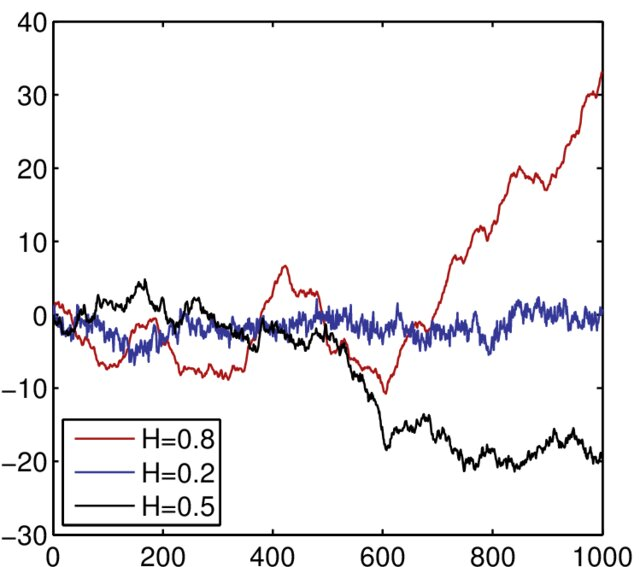
\includegraphics[scale=0.95]{fbm2.jpg}
		\caption{\footnotesize simulacije FBM za različite \( H \) (\cite{fracizvor})}
	\end{figure}
\end{frame}

\begin{frame}{Integralne reprezentacije FBM}
	Mandelbrot--van Ness:
	\begin{equation}
		B^H_t \jpod \int_\R \left[ (t-u)_+^{H-1/2}-(-u)_+^{H-1/2} \right] \D B_u, \quad t \ge 0.
	\end{equation}
	\vskip20pt
	Harmonizabilna reprezentacija:
	\begin{equation}
		B_t^H \jpod \int_\R \frac{e^{it\xi}-1}{(i\xi)^{H+1/2}} \D \wh B_\xi, \quad t \ge 0.
	\end{equation}
\end{frame}

\section{\holder -regularnost}
\begin{frame}{Uniformna \holder-regularnost na kompaktnom skupu}
	\textbf{Teorem.} Za svaki \( \alpha \in \left\langle0,H\right\rangle \) FBM ima modifikaciju
	\( \left\{ \wt B_t^H \right\} \) takvu da
	\begin{equation}
		\sup_{0 \le s,t \le T} \frac{\abs{\wt B_t^H - \wt B_s^H}}{\abs{t-s}^\alpha} < \infty, \quad T \ge 0.
	\end{equation}

	\vskip20pt
	\textbf{Teorem.} Trajektorije FBM ne zadovoljavaju \holder ov uvjet u smislu prošlog teorema ni
	za koji \( \alpha > H \).
\end{frame}

\begin{frame}{\holder -regularnost po točkama}
	\textbf{Definicija.}
	Neka je \( \left\{ X_t \st t \in \R\right\} \) slučajni proces čije su trajektorije g.s.\
	lokalno ograničene i nigdje diferencijabilne. Za proizvoljni
	\( t_0 \in \R \) definira se \emph{kritični točkovni \holder ov eksponent} u \( t_0 \)
	\begin{equation}
		\alpha_{t_0} = \sup \left\{ \alpha > 0 \st
		\limsup\limits_{h \rightarrow 0} \frac{\abs{X_{t_0+h}-X_{t_0}}}{\abs h^\alpha} = 0
		\right\}.
	\end{equation}

	\vskip20pt
	\textbf{Teorem.} Za FBM g.s.\ vrijedi \( \alpha_{t_0} = H \) za sve \( t_0 \in \R \).

\end{frame}

\section{Rješenje problema \holder -regularnosti po točkama}
\begin{frame}{Funkcije \( \Psi_{\pm H} \)}
	Neka je \( \psi \) Meyerov matični valić. Definiramo
	\begin{align}
		\Psi_H(x)    & = \int_\R
		e^{ix\xi} \frac{\wh \psi(\xi)}{(i\xi)^{H+1/2}} \D \xi, \\
		\Psi_{-H}(x) & = \int_\R e^{ix\xi} \wh \psi(\xi)
		(-i\xi)^{H+1/2} \D \xi, \quad x \in \R.
	\end{align}

	\vskip20pt
	Vrijedi
	\begin{equation}
		\int_\R \Psi_{-H}(t) \D t = \int_\R \Psi_H(t) \D t = 0.
	\end{equation}
	\begin{equation}\label{eq:intpsihpsi-h}
		2^{(j'+j)/2}\int_\R \Psi_H(2^{j'}t-k')\Psi_{-H}(2^jt-k) \D t =
		\begin{cases}
			1, \  & (j,k)=(j',k') \\
			0, \  & \text{inače}.
		\end{cases}
	\end{equation}
\end{frame}

\begin{frame}{Valićna reprezentacija FBM}
	\textbf{Teorem.} Neka je
	\begin{equation}
		B_t^H = \int_\R \frac{e^{it\xi}-1}{(i\xi)^{H+1/2}} \D \wh B_\xi, \quad t \in \R
	\end{equation}
	i \( \varepsilon_{j,k} \stackrel{\mathrm{n.j.d.}}{\sim} \mathrm N(0,1) \) definirane sa
	\begin{equation}
		\varepsilon_{j,k} =
		\int_\R 2^{-j/2}e^{ik2^{-j}\xi}\wh \psi(-2^{-j}\xi)\D \wh B_\xi =
		\int_\R 2^{j/2} \psi(2^jt-k) \D B_t.
	\end{equation}
	Tada je
	\begin{equation}\label{eq:valfbmrep}
		B^H_t = \sum_{j,k \in \Z}
		2^{-jH} \left( \Psi_H(2^jt - k) - \Psi_H(-k)  \right) \varepsilon_{j,k}, \quad t \in \R
	\end{equation}
	pri čemu konvergencija vrijedi i g.s.\ uniformno po \( t \) na svakom
	kompaktnom podskupu od \( \R \).
\end{frame}

\begin{frame}[allowframebreaks]{Put do glavnog rezultata}
	\textbf{Definicija.} Za \( j \in \N \) i \( \ell \in \Z \) označimo
	\begin{equation}
		\nu_j^\ell = \max \left\{ \abs{\varepsilon_{j,j\ell+m}} \st 0 \le m \le j-1 \right\}.
	\end{equation}

	\vskip10pt
	\textbf{Lema.} Gotovo sigurno iz \( \alpha_{t_0}(\omega_0) > H \) slijedi
	\begin{equation}
		\limsup\limits_{j \ub} \nu_j^{\ell_j(t_0)}(\omega_0) = 0
	\end{equation}
	gdje \( \ell_j(t_0) = \max\left\{ \ell \in \Z \st j\ell \le 2^jt_0 \right\} \).

	\vskip10pt
	Za dokaz se koristi ova formula inverzije:
	\begin{equation}
		\varepsilon_{j,k} = 2^{j(1+H)}\int_\R B^H_t\Psi_{-H}(2^jt-k) \D t \mathgs
	\end{equation}

	\framebreak
	\textbf{Lema.} Gotovo sigurno za sve \( p \in \Z \) vrijedi
	\begin{equation}
		\liminf\limits_{j \ub} \min \left\{ \nu_j^\ell(\omega) \st
		(p-1)2^j \le j\ell \le (p+1)2^j \right\} \ge \frac 12.
	\end{equation}
\end{frame}


\begin{frame}[t, allowframebreaks]{Bibliografija}
	\printbibliography
\end{frame}
\end{document}
